\chapter{Systems} \label{chp:systems}
\epigraph{We must be clear that when it comes to atoms, language can be used only as in poetry.}{Niels Bohr, \cite{heisenberg_physics_1971}}
\begin{figure}[H]
	\centering
	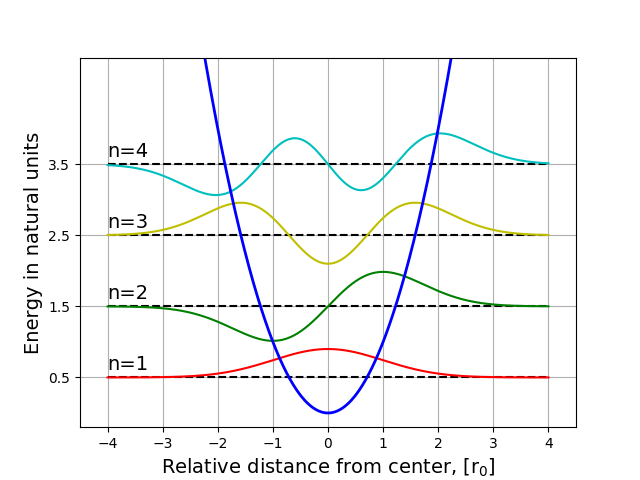
\includegraphics[scale=0.9]{Images/harmonicOscillator.png}
	\caption{The quantum harmonic oscillator, with the Hermite functions represented up to 4th order. As in classical mechanics, the harmonic oscillator can describe various quantum systems, such as lattice vibration (phonons) and quantum fields.}
	\label{fig:harmonicoscillator}
\end{figure}

When defining a system, we also need to specify the basis set to be used. The single particle functions are often known, and they are well-suited as a basis for the total

\newpage
\section{Quantum dots} \label{subsubsec:quantumdots}
Quantum dots are very small particles, and contain fermions or bosons hold together by an external potential. Since these particles have discrete electronic states like an atom, they are often called artificial atoms. 

In this thesis we will, among other systems, study electrons trapped in harmonic oscillators, where the external potential affecting particle $i$ is given by
\begin{equation}
u_i=\frac{1}{2}m\omega^2r_i^2.
\end{equation}
where $m$ is the mass of particle $i$, $\omega$ is the oscillator frequency and $r_i$ is the relative distance from particle $i$ to the center of the trap. 

Using natural units as described in Appendix B, we can write the Hamiltonian as
\begin{equation}
\label{eq:HOHamiltonian}
\hat{\mathcal{H}} = \sum_{i=1}^{P} \Big(-\frac{1}{2} \nabla_i^2 + \frac{1}{2} \omega^2r_i ^2\Big) + \sum_{i<j} \frac{1}{r_{ij}} 
\end{equation}
where the energy is scaled with respect to atomic units and lengths are scaled with respect to the Bohr radius.

The exact solutions of the non-interacting Hamiltonian are the Hermite functions, 
\begin{equation}
\phi_n(x)=H_n(\sqrt{\omega}x)\exp(-\omega x^2/2)
\end{equation}
which can be used as the basis. $H_n(x)$ is the Hermite polynomial of $n$'th degree, and the first four Hermite functions are illustrated in figure \eqref{fig:harmonicoscillator}. The energy of a particle at energy level $n$ in a $D$ dimensional harmonic oscillator is given by
\begin{equation}
E_n=\omega\Big(n+\frac{D}{2}\Big).
\label{eq:HOenergies}
\end{equation}

We will study closed-shell systems only, since the Slater determinant in that case is unambiguous. For open shells, the total Slater determinant is a linear combination of all the possible Slater determinants. The number of particles of closed-shell systems are called magic numbers, which in two dimensions are $N=2,6,12,\hdots$. In general, the magic numbers are given by
\begin{equation}
N=s\binom{n+D}{D}
\label{eq:HOclosedshell}
\end{equation}
where $s$ is the number of spin configurations (2), $n$ is the principal quantum number and $d$ is the number of dimensions. This is a direct consequence of the Pauli principle, where we in the ground state can have two particles with radial wave functions $\Phi_{n_x=0,n_y=0}$, in the next energy level we have have 4 particles with radial wave functions $\Phi_{n_x=1,n_y=0}$ and $\psi_{n_x=0,n_y=1}$ with degeneracy 2 and so on. 

\begin{figure}
	\begin{center}
		\begin{tikzpicture}[scale=0.7]
		\begin{scope}
		\foreach \i in {0,...,3}
		{
			\draw (-1,\i) node[anchor=east] {$\i$} --(2,\i);
		}
		\filldraw[color=color0] (0,0) node[anchor=north,inner sep=.4cm, color=black] {$n_x$} circle (0.25cm); 
		\filldraw[color=color0] (1,0) node[anchor=north,inner sep=.4cm, color=black] {$n_y$} circle (0.25cm);
		\node[] at (0.5,3.8) {$n=0$};
		\end{scope}
		\begin{scope}[xshift=5cm]
		\foreach \i in {0,...,3}
		{
			\draw (-1,\i) --(2,\i);
		}
		\draw[color=color1] (0,0) node[anchor=north,inner sep=.4cm, color=black] {$n_x$} circle (0.25cm); 
		\filldraw[color=color0] (1,0) node[anchor=north,inner sep=.4cm, color=black] {$n_y$} circle (0.25cm);
		\filldraw[color=color0] (0,3) circle (0.25cm);
		\end{scope}
		\begin{scope}[xshift=9cm]
		\foreach \i in {0,...,3}
		{
			\draw (-1,\i) --(2,\i);
		}
		\draw[color=color1] (0,0) node[anchor=north,inner sep=.4cm, color=black] {$n_x$} circle (0.25cm); 
		\draw[color=color1] (1,0) node[anchor=north,inner sep=.4cm, color=black] {$n_y$} circle (0.25cm);
		\filldraw[color=color0] (0,2) circle (0.25cm); 
		\filldraw[color=color0] (1,1) circle (0.25cm); 
		\node[] at (2.5,3.8) {$n=3$};
		\end{scope}
		\begin{scope}[xshift=13cm]
		\foreach \i in {0,...,3}
		{
			\draw (-1,\i) --(2,\i);
		}
		\draw[color=color1] (0,0) node[anchor=north,inner sep=.4cm, color=black] {$n_x$} circle (0.25cm); 
		\draw[color=color1] (1,0) node[anchor=north,inner sep=.4cm, color=black] {$n_y$} circle (0.25cm);
		\filldraw[color=color0] (0,1) circle (0.25cm); 
		\filldraw[color=color0] (1,2) circle (0.25cm); 
		\end{scope}
				\begin{scope}[xshift=17cm]
		\foreach \i in {0,...,3}
		{
			\draw (-1,\i) --(2,\i);
		}
		\filldraw[color=color0] (0,0) node[anchor=north,inner sep=.4cm, color=black] {$n_x$} circle (0.25cm); 
		\draw[color=color1] (1,0) node[anchor=north,inner sep=.4cm, color=black] {$n_y$} circle (0.25cm);
		\filldraw[color=color0] (1,3) circle (0.25cm); 
		\end{scope}
		\end{tikzpicture}
	\end{center}

	\begin{center}
		\begin{tikzpicture}[scale=0.7]
		\begin{scope}
		\foreach \i in {0,...,3}
		{
			\draw (-1,\i) node[anchor=east] {$\i$} --(2,\i);
		}
		\draw[color=color1] (0,0) node[anchor=north,inner sep=.4cm, color=black] {$n_x$} circle (0.25cm); 
		\filldraw[color=color0] (1,0) node[anchor=north,inner sep=.4cm, color=black] {$n_y$} circle (0.25cm);
		\filldraw[color=color0] (0,1) circle (0.25cm);
		\node[] at (2.5,3.8) {$n=1$};
		\end{scope}
		\begin{scope}[xshift=4cm]
		\foreach \i in {1,...,4}
		{
			\draw (-1,\i-1) --(2,\i-1);
		}
		\filldraw[color=color0] (0,0) node[anchor=north,inner sep=.4cm, color=black] {$n_x$} circle (0.25cm); 
		\draw[color=color1] (1,0) node[anchor=north,inner sep=.4cm, color=black] {$n_y$} circle (0.25cm);
		\filldraw[color=color0] (1,1) circle (0.25cm); 
		\end{scope}
		\begin{scope}[xshift=9cm]
		\foreach \i in {1,...,4}
		{
			\draw (-1,\i-1) --(2,\i-1);
		}
		\draw[color=color1] (0,0) node[anchor=north,inner sep=.4cm, color=black] {$n_x$} circle (0.25cm); 
		\filldraw[color=color0] (1,0) node[anchor=north,inner sep=.4cm, color=black] {$n_y$} circle (0.25cm);
		\filldraw[color=color0] (0,2) circle (0.25cm);
		\end{scope}
		\begin{scope}[xshift=13cm]
		\foreach \i in {1,...,4}
		{
			\draw (-1,\i-1) --(2,\i-1);
		}
		\draw[color=color1] (0,0) node[anchor=north,inner sep=.4cm, color=black] {$n_x$} circle (0.25cm); 
		\draw[color=color1] (1,0) node[anchor=north,inner sep=.4cm, color=black] {$n_y$} circle (0.25cm);
		\filldraw[color=color0] (0,1) circle (0.25cm); 
		\filldraw[color=color0] (1,1) circle (0.25cm);
		\node[] at (0.5,3.8) {$n=2$};
		\end{scope}
		\begin{scope}[xshift=17cm]
		\foreach \i in {1,...,4}
		{
			\draw (-1,\i-1) --(2,\i-1);
		}
		\filldraw[color=color0] (0,0) node[anchor=north,inner sep=.4cm, color=black] {$n_x$} circle (0.25cm); 
		\draw[color=color1] (1,0) node[anchor=north,inner sep=.4cm,color=black] {$n_y$} circle (0.25cm); 
		\filldraw[color=color0] (1,2) circle (0.25cm);
		\end{scope}
		\end{tikzpicture}
	\end{center}
	\caption{The possible states of a two-dimensional quantum dot for $n=n_x+n_y=0,1,2,3$. Recalling that the electrons can take spins $+1$ and $-1$, one can use this schematic to determine the maximal number of electrons in each shell and thus reveal the magic numbers.}
	\label{fig:hostates}
\end{figure}
\begin{figure} [H]
	\begin{center}
		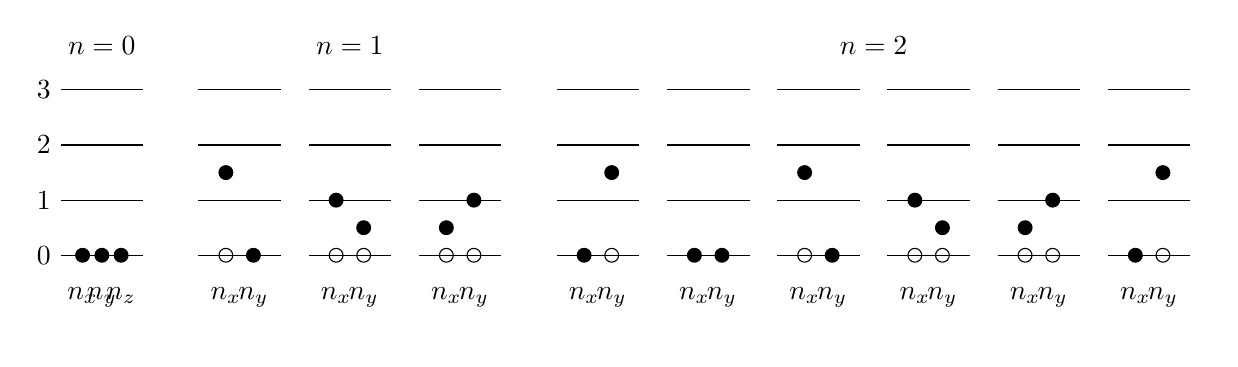
\begin{tikzpicture}[scale=0.35]
		\begin{scope}
		\foreach \i in {0,...,3}
		{
			\draw (-1,2*\i) node[anchor=east] {$\i$} --(2,2*\i);
		}
		\filldraw (-0.2,0) node[anchor=north,inner sep=.4cm] {$n_x$} circle (0.25cm); 
		\filldraw (0.5,0) node[anchor=north,inner sep=.4cm] {$n_y$} circle (0.25cm);
		\filldraw (1.2,0) node[anchor=north,inner sep=.4cm] {$n_z$} circle (0.25cm);
		\node[] at (0.5,7.6) {$n=0$};
		\end{scope}
		\begin{scope}[xshift=5cm]
		\foreach \i in {0,...,3}
		{
			\draw (-1,2*\i) --(2,2*\i);
		}
		\draw (0,0) node[anchor=north,inner sep=.4cm] {$n_x$} circle (0.25cm); 
		\filldraw (1,0) node[anchor=north,inner sep=.4cm] {$n_y$} circle (0.25cm);
		\filldraw (0,3) circle (0.25cm);
		\end{scope}
		\begin{scope}[xshift=9cm]
		\foreach \i in {0,...,3}
		{
			\draw (-1,2*\i) --(2,2*\i);
		}
		\draw (0,0) node[anchor=north,inner sep=.4cm] {$n_x$} circle (0.25cm); 
		\draw (1,0) node[anchor=north,inner sep=.4cm] {$n_y$} circle (0.25cm);
		\filldraw (0,2) circle (0.25cm); 
		\filldraw (1,1) circle (0.25cm); 
		\node[] at (0.5,7.6) {$n=1$};
		\end{scope}
		\begin{scope}[xshift=13cm]
		\foreach \i in {0,...,3}
		{
			\draw (-1,2*\i) --(2,2*\i);
		}
		\draw (0,0) node[anchor=north,inner sep=.4cm] {$n_x$} circle (0.25cm); 
		\draw (1,0) node[anchor=north,inner sep=.4cm] {$n_y$} circle (0.25cm);
		\filldraw (0,1) circle (0.25cm); 
		\filldraw (1,2) circle (0.25cm); 
		\end{scope}
		\begin{scope}[xshift=18cm]
		\foreach \i in {0,...,3}
		{
			\draw (-1,2*\i) --(2,2*\i);
		}
		\filldraw (0,0) node[anchor=north,inner sep=.4cm] {$n_x$} circle (0.25cm); 
		\draw (1,0) node[anchor=north,inner sep=.4cm] {$n_y$} circle (0.25cm);
		\filldraw (1,3) circle (0.25cm); 
		\end{scope}
		\begin{scope}[xshift=22cm]
		\foreach \i in {0,...,3}
		{
			\draw (-1,2*\i) --(2,2*\i);
		}
		\filldraw (0,0) node[anchor=north,inner sep=.4cm] {$n_x$} circle (0.25cm); 
		\filldraw (1,0) node[anchor=north,inner sep=.4cm] {$n_y$} circle (0.25cm);
		\end{scope}
		\begin{scope}[xshift=26cm]
		\foreach \i in {0,...,3}
		{
			\draw (-1,2*\i) --(2,2*\i);
		}
		\draw (0,0) node[anchor=north,inner sep=.4cm] {$n_x$} circle (0.25cm); 
		\filldraw (1,0) node[anchor=north,inner sep=.4cm] {$n_y$} circle (0.25cm);
		\filldraw (0,3) circle (0.25cm);
		\node[] at (2.5,7.6) {$n=2$};
		\end{scope}
		\begin{scope}[xshift=30cm]
		\foreach \i in {0,...,3}
		{
			\draw (-1,2*\i) --(2,2*\i);
		}
		\draw (0,0) node[anchor=north,inner sep=.4cm] {$n_x$} circle (0.25cm); 
		\draw (1,0) node[anchor=north,inner sep=.4cm] {$n_y$} circle (0.25cm);
		\filldraw (0,2) circle (0.25cm); 
		\filldraw (1,1) circle (0.25cm); 
		\end{scope}
		\begin{scope}[xshift=34cm]
		\foreach \i in {0,...,3}
		{
			\draw (-1,2*\i) --(2,2*\i);
		}
		\draw (0,0) node[anchor=north,inner sep=.4cm] {$n_x$} circle (0.25cm); 
		\draw (1,0) node[anchor=north,inner sep=.4cm] {$n_y$} circle (0.25cm);
		\filldraw (0,1) circle (0.25cm); 
		\filldraw (1,2) circle (0.25cm); 
		\end{scope}
		\begin{scope}[xshift=38cm]
		\foreach \i in {0,...,3}
		{
			\draw (-1,2*\i) --(2,2*\i);
		}
		\filldraw (0,0) node[anchor=north,inner sep=.4cm] {$n_x$} circle (0.25cm); 
		\draw (1,0) node[anchor=north,inner sep=.4cm] {$n_y$} circle (0.25cm);
		\filldraw (1,3) circle (0.25cm); 
		\end{scope}
		\end{tikzpicture}
	\end{center}

	\begin{center}
		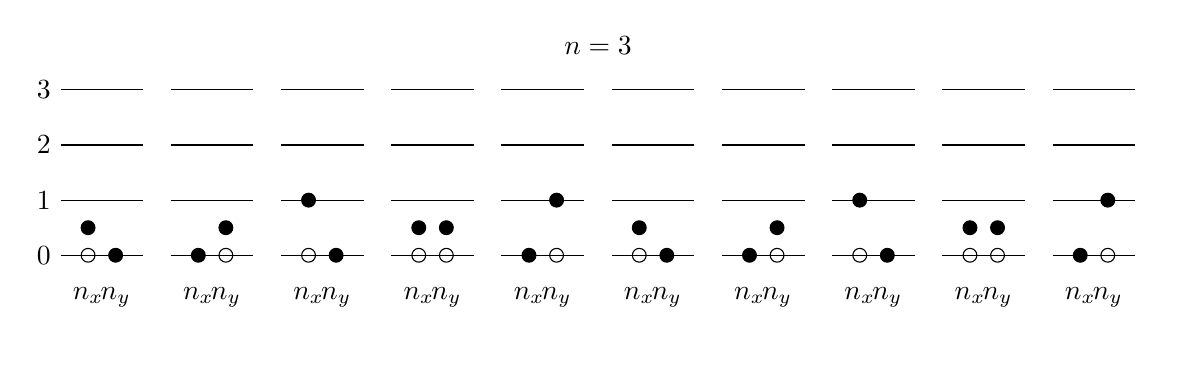
\begin{tikzpicture}[scale=0.35]
		\begin{scope}
		\foreach \i in {0,...,3}
		{
			\draw (-1,2*\i) node[anchor=east] {$\i$} --(2,2*\i);
		}
		\draw (0,0) node[anchor=north,inner sep=.4cm] {$n_x$} circle (0.25cm); 
		\filldraw (1,0) node[anchor=north,inner sep=.4cm] {$n_y$} circle (0.25cm);
		\filldraw (0,1) circle (0.25cm);
		\end{scope}
		\begin{scope}[xshift=4cm]
		\foreach \i in {0,...,3}
		{
			\draw (-1,2*\i) --(2,2*\i);
		}
		\filldraw (0,0) node[anchor=north,inner sep=.4cm] {$n_x$} circle (0.25cm); 
		\draw (1,0) node[anchor=north,inner sep=.4cm] {$n_y$} circle (0.25cm);
		\filldraw (1,1) circle (0.25cm); 
		\end{scope}
		\begin{scope}[xshift=8cm]
		\foreach \i in {0,...,3}
		{
			\draw (-1,2*\i) --(2,2*\i);
		}
		\draw (0,0) node[anchor=north,inner sep=.4cm] {$n_x$} circle (0.25cm); 
		\filldraw (1,0) node[anchor=north,inner sep=.4cm] {$n_y$} circle (0.25cm);
		\filldraw (0,2) circle (0.25cm);
		\end{scope}
		\begin{scope}[xshift=12cm]
		\foreach \i in {0,...,3}
		{
			\draw (-1,2*\i) --(2,2*\i);
		}
		\draw (0,0) node[anchor=north,inner sep=.4cm] {$n_x$} circle (0.25cm); 
		\draw (1,0) node[anchor=north,inner sep=.4cm] {$n_y$} circle (0.25cm);
		\filldraw (0,1) circle (0.25cm); 
		\filldraw (1,1) circle (0.25cm);
		\end{scope}
		\begin{scope}[xshift=16cm]
		\foreach \i in {0,...,3}
		{
			\draw (-1,2*\i) --(2,2*\i);
		}
		\filldraw (0,0) node[anchor=north,inner sep=.4cm] {$n_x$} circle (0.25cm); 
		\draw (1,0) node[anchor=north,inner sep=.4cm] {$n_y$} circle (0.25cm); 
		\filldraw (1,2) circle (0.25cm);
		\node[] at (2.5,7.6) {$n=3$};
		\end{scope}
		\begin{scope}[xshift=20cm]
		\foreach \i in {0,...,3}
		{
			\draw (-1,2*\i) --(2,2*\i);
		}
		\draw (0,0) node[anchor=north,inner sep=.4cm] {$n_x$} circle (0.25cm); 
		\filldraw (1,0) node[anchor=north,inner sep=.4cm] {$n_y$} circle (0.25cm);
		\filldraw (0,1) circle (0.25cm);
		\end{scope}
		\begin{scope}[xshift=24cm]
		\foreach \i in {0,...,3}
		{
			\draw (-1,2*\i) --(2,2*\i);
		}
		\filldraw (0,0) node[anchor=north,inner sep=.4cm] {$n_x$} circle (0.25cm); 
		\draw (1,0) node[anchor=north,inner sep=.4cm] {$n_y$} circle (0.25cm);
		\filldraw (1,1) circle (0.25cm); 
		\end{scope}
		\begin{scope}[xshift=28cm]
		\foreach \i in {0,...,3}
		{
			\draw (-1,2*\i) --(2,2*\i);
		}
		\draw (0,0) node[anchor=north,inner sep=.4cm] {$n_x$} circle (0.25cm); 
		\filldraw (1,0) node[anchor=north,inner sep=.4cm] {$n_y$} circle (0.25cm);
		\filldraw (0,2) circle (0.25cm);
		\end{scope}
		\begin{scope}[xshift=32cm]
		\foreach \i in {0,...,3}
		{
			\draw (-1,2*\i) --(2,2*\i);
		}
		\draw (0,0) node[anchor=north,inner sep=.4cm] {$n_x$} circle (0.25cm); 
		\draw (1,0) node[anchor=north,inner sep=.4cm] {$n_y$} circle (0.25cm);
		\filldraw (0,1) circle (0.25cm); 
		\filldraw (1,1) circle (0.25cm);
		\end{scope}
		\begin{scope}[xshift=36cm]
		\foreach \i in {0,...,3}
		{
			\draw (-1,2*\i) --(2,2*\i);
		}
		\filldraw (0,0) node[anchor=north,inner sep=.4cm] {$n_x$} circle (0.25cm); 
		\draw (1,0) node[anchor=north,inner sep=.4cm] {$n_y$} circle (0.25cm); 
		\filldraw (1,2) circle (0.25cm);
		\end{scope}
		\end{tikzpicture}
	\end{center}
	\caption{Possible states of a three dimensional harmonic oscillator.}
	\label{fig:schematic_3d}
\end{figure}

\section{Atomic systems} \label{subsubsec:atomic}
We will also investigate real atoms, where we freeze out the nucleonic degrees of freedom known as the Born-Oppenheimer approximation. The electrons will in fact affect the nucleus, but due to the mass difference this effect will be negligible.

We again have Coulomb interaction between the electrons and the nucleus, and since we assume the latter to be at rest at the origin, the external potential affecting particle $i$ is
\begin{equation}
u_i=- \frac{1}{2} k\frac{Ze^2}{r_i},
\end{equation}
where $Z$ is the atomic number (number of protons inside the nucleus). The total Hamiltonian is given in (Hartree) atomic units, 
\begin{equation}
\label{eq:AtomicHamiltonian}
\hat{\mathcal{H}} = \sum_{i=1}^{P} \Big(-\frac{1}{2} \nabla_i^2 - \frac{1}{2} \frac{Z}{r_i}+\frac{l(l+1)}{2r_i^2}\Big) + \sum_{i<j} \frac{1}{r_{ij}},
\end{equation}
which also is discussed in Appendix B. For the non-interacting case, the energies are given by the Bohr formula
\begin{equation}
E_n=-\frac{Z^2}{2n^2}.
\label{eq:bohrformula}
\end{equation}

For atomic systems, it is convenient to use spherical coordinates, which allows us to split up the wave function in a radial part and an angular part,
\begin{equation}
\psi_{nlm}(r,\theta,\phi)=R_{nl}(r)Y_l^m(\theta,\phi)
\end{equation}

The exact radial part for the non-interacting case is called the hydrogen-like orbitals, that is
\begin{equation}
R_{nl}(r)\propto r^le^{-Zr/n}\Big[L_{n-l-1}^{2l+1}\Big(\frac{2r}{n}Z\Big)\Big]
\end{equation}
where $L_{q}^p(x)$ are the \textit{associated Laguerre polynomials} or \textit{generalized Laguerre polynomials}. More about them and how to calculate them recursively can be found in Appendix C. 

The angular part is given by the \textit{spherical harmonics}
\begin{equation}
Y_l^m(\theta,\phi)\propto P_l^m(\cos\theta)e^{im\phi}
\end{equation}
where $P_l^m(x)$ are the \textit{associated Legendre polynomials}. The complex part in the spherical harmonics causes some difficulties, and we will therefore instead use the solid harmonics
\begin{equation}
\label{eq:V_ext}
S_l^m(r,\theta,\phi)\propto r^lP_l^{|m|}(\cos\theta)
\begin{cases} 
\cos(m\phi) & \text{if} \quad m\geq0 \\
\sin(|m|\phi) & \text{if} \quad m<0.
\end{cases}
\end{equation}

Again we will study closed shells only, but for atoms we will introduce subshells as well, which are dependent on the azimuthal quantum number $l$ in addition to the principal quantum number $n$. In general, we have that $l\in [0,n-1]$ such that we only have one subshell for $n=1$. Traditionally, the first few subshells are denoted with $s, p, d$ and $f$, and the meaning can be found in table \eqref{tab:subshells}, together with number of electrons in each subshell.

\begin{table} [H]
	\caption{Table of the first subshells  \vspace{2mm}}
	\begin{tabularx}{\textwidth}{X|X:X:X} \hline\hline
		\label{tab:subshells}
		Subshell label & $l$ & Max electrons & Name \\ \hline
		$s$ & 0 & 2 & sharp\\ 
		$p$ & 1 & 6 & principal\\
		$d$ & 2 & 10 & diffuse \\
		$f$ & 3 & 14 & fundamental \\
		$g$ & 4 & 18 & alphabetic \\ \hline\hline
	\end{tabularx}
\end{table}

For Helium, we have two electrons with $n=1$, which means that both have $l=0$ and both electrons are in the $s$-subshell. We can thus write the electron configuration as $1s^2$. 

Similar as for the principal quantum number $n$, we can use the tumble rule the lower $l$ the lower energy, such that for Beryllium all four electrons are still in the $s$-subshell. Beryllium therefore has electron configuration $1s^2 2s^2$ or [He] $2s^2$. Since both subshells are fully occupied, Beryllium can be included in our closed-shell calculations. 

If we continue with the same rules, we see that the next closed-shell atom has a fully occupied $p$-subshell as well, which is Neon with 10 electrons. This is a noble gas, and we can write the electron configuration as [Be] $2p^6$. All noble gases have endings $Xs^2 Xp^6$, which is the reason why they always have 8 valence electrons.

We can now compare this to the periodical system, and observe that the two first rows agrees with the theory presented above: The first row has two elements and the second has eight. However, the third one also has eight elements, which does not fit our theory. The reason is that the angular momentum contribution is not taken into account, i.e., we need to include the Hamiltonian term
\begin{equation}
V_L=\frac{l(l+1)}{2r^2}
\end{equation}
as well. If we do so, we see that the thumb rule defined above not always holds. Sometimes a low $l$ in a higher $n$ causes lower energy than a high $l$ in a lower $n$. 

"Colloquially, we call such solutions and derived properties as electronic structure."

\section{Molecular systems}
For molecular systems the same principles applies as for an atom, but we now have multiple contributions to the external potential. 

\section{Bose-Einstein Condensation}
Already in 1925, A. Einstein predicted that all bosons occupy the same quantum state for temperatures close to the absolute zero. [NEED REFERENCE, Bose–Einstein Condensation in Dilute Gases] It would take 70 years for someone to come up with an experiment to prove the prediction, when M.H. Andersen et.al. managed reach those extreme temperatures using laser cooling. [NEED REFERENCE, Observation of bose-einstein condensation in a dilute atomic vapor.]

The bosons do not interact with the Coulomb interaction as we have seen above: The actual interaction is unknown, but we can model it with a hard-sphere potential...

